\documentclass[aspectratio=169]{beamer}

% Tema visual
\usetheme{Madrid}
\usecolortheme{whale}

% Paquetes necesarios
\usepackage[utf8]{inputenc}
\usepackage[spanish]{babel}
\usepackage{amsmath, amssymb}
\usepackage{graphicx}
\usepackage{booktabs}
\usepackage{tikz} % Útil para diagramas ópticos si decides dibujarlos después

% Información de la presentación
\title[Calibración FPP]{Método de Calibración Flexible para \\ Profilometría de Proyección de Franjas (FPP)}
\subtitle{Modelo Rayo-Fase y Calibración Estéreo Asistida}
\author[Rojas Martínez, J. F.]{Jonathan Francisco Rojas Martínez \\ \footnotesize Basado en Y. Lyu et al.}
\institute[CIO]{Centro de Investigaciones en Óptica}
\date{\today}

\begin{document}
	
	% Diapositiva de Título
	\begin{frame}
		\titlepage
	\end{frame}
	
	% ------------------ INTRODUCCIÓN ------------------
	\section{Introducción}
	
	\begin{frame}{Metrología Óptica 3D y FPP}
		\begin{columns}
			\begin{column}{0.55\textwidth}
				\begin{itemize}
					\item La \textbf{Profilometría de Proyección de Franjas (FPP)} es una técnica de percepción 3D basada en luz estructurada.
					\item \textbf{Principio:} Codifica el volumen de medición proyectando patrones sinusoidales; la topografía del objeto deforma físicamente la fase óptica.
					\%item \textbf{Ventajas frente a CMM:} 
					%\begin{itemize}
						%\item Naturaleza sin contacto.
						%\item Adquisición de campo completo de alta densidad.
					%\end{itemize}
				\end{itemize}
			\end{column}
			\begin{column}{0.45\textwidth}
				\begin{figure}[htbp]
					\centering
					% Ajusta el ancho al tamaño de la columna (\textwidth) o a una medida específica como 4cm
					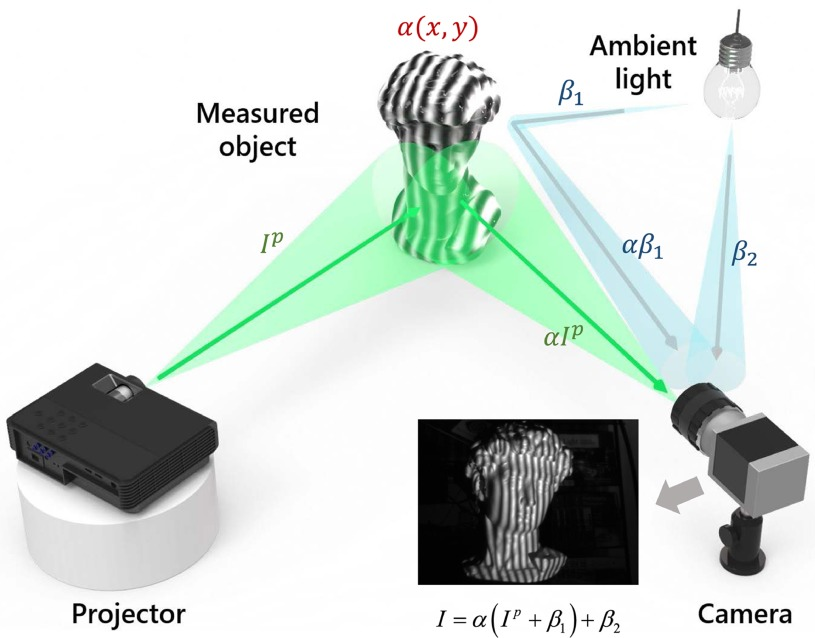
\includegraphics[width=0.8\textwidth]{FPP_general.jpg} 
					\vspace{0.2cm} % Un pequeño espacio entre la imagen y la leyenda
					\caption{FPP general.}
					\label{fig:mi_etiqueta}
				\end{figure}
			\end{column}
		\end{columns}
	\end{frame}
	
	\begin{frame}{El Cuello de Botella: La Calibración Clásica}
		\begin{block}{El Objetivo de la Calibración}
			Establecer la relación matemática exacta entre la información del campo de luz (fase) y las coordenadas físicas 3D $(x,y,z)$.
		\end{block}
		
		\begin{alertblock}{Limitaciones de los métodos tradicionales}
			\begin{itemize}
				\item Dependencia de hardware altamente preciso y costoso (platinas de traslación $Z$, bloques patrón).
				\item Necesidad de realizar \textbf{interpolaciones espaciales} de fase sobre los marcadores (ej. esquinas de un tablero de ajedrez), lo que induce errores numéricos.
			\end{itemize}
		\end{alertblock}
	\end{frame}
	
	% ------------------ FUNDAMENTOS Y MATEMÁTICAS ------------------
	\section{Fundamentos Físicos}
	
	\begin{frame}{Recuperación de la Fase (Phase-Shifting)}
		\begin{columns}
			\begin{column}{0.6\textwidth}
				La intensidad capturada $I_n(x,y)$ en un algoritmo de desplazamiento de fase ($N$ pasos) se modela como:
				\begin{equation*}
					I_{n}(x,y) = b(x,y) + m(x,y)\cos\left[\varphi(x,y) + \frac{2n\pi}{N}\right]
				\end{equation*}
				
				Aplicando ortogonalidad trigonométrica (mínimos cuadrados), aislamos la fase relativa:
				\begin{equation*}
					\varphi_{env}(x,y) = \arctan \left( \frac{\sum_{n=1}^{N} I_n \sin(2n\pi/N)}{\sum_{n=1}^{N} I_n \cos(2n\pi/N)} \right)
				\end{equation*}
			\end{column}
			\begin{column}{0.4\textwidth}
				\begin{itemize}
					\item $b(x,y)$: Iluminación de fondo.
					\item $m(x,y)$: Modulación/Contraste.
					\item $\varphi(x,y)$: \textbf{Fase buscada}.
				\end{itemize}
				
			\end{column}
		\end{columns}
	\end{frame}
	
	\begin{frame}{Desenvolvimiento de Fase (TPU) y Cámara Virtual}
		\begin{columns}
			\begin{column}{0.5\textwidth}
				\textbf{1. Desenvolvimiento Temporal (TPU)}
				\begin{itemize}
					\item La función arctan produce saltos de fase (fase envuelta $[-\pi, \pi]$).
					\item Se aplica un Desenvolvimiento de Fase Temporal (TPU) para obtener la \textbf{fase absoluta continua} $\varphi$, vinculándola a una profundidad única.
				\end{itemize}
			\end{column}
			\begin{column}{0.5\textwidth}
				\textbf{2. Corrección de Distorsión}
				\begin{itemize}
					\item Los modelos matemáticos de propagación asumen líneas rectas.
					\item Se pre-calibra el lente para corregir matemáticamente su distorsión.
					\item Esto genera una \textbf{cámara virtual estenopeica} idealizada sobre la cual operará el modelo.
				\end{itemize}
			\end{column}
		\end{columns}
	\end{frame}
	
	\begin{frame}{El Modelo Rayo-Fase (Ray-Phase Model)}
		\begin{columns}
			\begin{column}{0.5\textwidth}
				A diferencia de mapear fase a altura $h(x,y)$, se utiliza el centro óptico de la cámara como origen $(x_c, y_c, z_c)$.
				\begin{itemize}
					\item Cada píxel corresponde a un \textbf{rayo de luz único}.
					\item La fase absoluta $\varphi$ crece de forma monótona a lo largo de este rayo ($z_c$).
				\end{itemize}
			\end{column}
			\begin{column}{0.5\textwidth}
				\begin{block}{Ecuaciones del Sistema}
					\begin{equation*}
						\begin{cases}
							x_c = A(i,j)z_c \\
							y_c = B(i,j)z_c \\
							z_c = \sum_{n=0}^{N} a_n(i,j)\varphi^n
						\end{cases}
					\end{equation*}
				\end{block}
				\small{$A, B$: Coeficientes directores del rayo.\\ $a_n$: Polinomio de profundidad-fase.}
			\end{column}
		\end{columns}
	\end{frame}
	
	% ------------------ DESARROLLO EXPERIMENTAL ------------------
	\section{Desarrollo Experimental}
	
	\begin{frame}{Procedimiento de Calibración: Paso 1 (Geometría Estéreo)}
		\begin{columns}
			\begin{column}{0.55\textwidth}
				\textbf{Introducción de una Cámara Auxiliar (B)}
				\begin{itemize}
					\item La Cámara A (medición) y la Cámara B forman un sistema de \textbf{Visión Estéreo Activa}.
					\item Se utiliza un patrón clásico (ajedrez/círculos) para calibrar intrínsecos de ambas cámaras y su geometría epipolar (Matriz de Rotación $R$ y Traslación $T$).
				\end{itemize}
			\end{column}
			\begin{column}{0.45\textwidth}
				\begin{figure}[htbp]
					\centering
					% Ajusta el ancho al tamaño de la columna (\textwidth) o a una medida específica como 4cm
					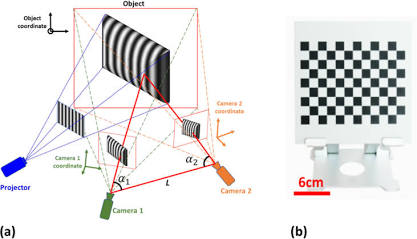
\includegraphics[width=0.8\textwidth]{estero_ctivo.jpeg} 
					\vspace{0.2cm} % Un pequeño espacio entre la imagen y la leyenda
					\caption{Vison estero activa}
					\label{DASDASD}
				\end{figure}
			\end{column}
		\end{columns}
	\end{frame}
	
	\begin{frame}{Procedimiento de Calibración: Paso 2 (Correspondencia por Fase)}
		\begin{columns}
			\begin{column}{0.4\textwidth}
				\textbf{Uso de un objeto liso y difuso (Cartulina)}
				\begin{itemize}
					\item El proyector emite patrones sobre la cartulina en 21 posiciones aleatorias.
					\item Al no haber textura, \textbf{la fase absoluta actúa como el rasgo (feature) para la correspondencia estéreo} entre la Cámara A y B.
					\item Esto permite triangular sub-píxel a sub-píxel las verdaderas coordenadas físicas $(x_c, y_c, z_c)$ \textbf{sin marcadores ni interpolación}.
				\end{itemize}
			\end{column}
			\begin{column}{0.6\textwidth}
				\begin{center}
					\begin{tikzpicture}[
						camera/.style={rectangle, draw=black, thick, fill=blue!10, minimum width=1.5cm, minimum height=1cm, text centered, rounded corners},
						projector/.style={rectangle, draw=black, thick, fill=orange!10, minimum width=1.8cm, minimum height=1cm, text centered, rounded corners},
						object/.style={rectangle, draw=black, thick, fill=gray!20, minimum width=5cm, minimum height=1.5cm, text centered},
						ray_proj/.style={->, thick, orange},
						ray_cam/.style={->, thick, dashed, blue}
						]
						
						% Definición de nodos (equipos)
						\node[camera] (camA) at (-3.5, 0) {Cámara A};
						\node[projector] (proj) at (0, 0) {Proyector};
						\node[camera] (camB) at (3.5, 0) {Cámara B};
						
						% Superficie de medición (sin textura)
						\node[object] (obj) at (0, 4) {Superficie lisa (ej. Cartulina blanca)};
						
						% Haces de luz del proyector (Patrón de franjas)
						\draw[ray_proj] (proj.north) -- (obj.south) node[midway, right, text=black] {Proyecta franjas};
						\draw[ray_proj] (proj.north) -- (-1.5, 3.25);
						\draw[ray_proj] (proj.north) -- (1.5, 3.25);
						
						% Haces de captura de las cámaras (Leyendo la fase)
						\draw[ray_cam] (0, 3.25) -- (camA.north) node[midway, left, text=black] {Captura fase \ \ };
						\draw[ray_cam] (0, 3.25) -- (camB.north) node[midway, right, text=black] {\ \ Captura fase};
						
						% Línea base estéreo
						\draw[<->, thick] (camA.south) -- (camB.south) node[midway, below] {Línea base conocida (Baseline)};
						
					\end{tikzpicture}
				\end{center}
			\end{column}
		\end{columns}
	\end{frame}
	
	\begin{frame}{Consolidación y Medición Final}
		\begin{block}{Ajuste de Mínimos Cuadrados}
			Para cada píxel $(i,j)$, se tienen múltiples pares de datos físicos y ópticos $\{z_{c,m}, \varphi_m\}$. Se aplica Mínimos Cuadrados para encontrar los coeficientes del polinomio $a_n(i,j)$.
		\end{block}
		
		\vspace{0.2cm}
		\textbf{Fase de Medición:}
		\begin{enumerate}
			\item La Cámara B se \textbf{retira} físicamente del sistema.
			\item Se proyectan las franjas sobre un objeto de interés y se calcula $\varphi$.
			\item Se inserta $\varphi$ en el polinomio específico del píxel para obtener $z_c$.
			\item Las constantes del rayo $A(i,j)$ y $B(i,j)$ determinan $x_c$ y $y_c$.
		\end{enumerate}
	\end{frame}
	
	% ------------------ CONCLUSIONES ------------------
	\section{Conclusiones}
	
	\begin{frame}{Resultados y Validación Metrológica}
		
				\begin{itemize}
					\item Evaluación reconstruyendo un plano físico mecanizado de precisión ($200\times160$ mm).
					\item \textbf{Cálculo de error:} Distancia de Euler desde la nube de puntos hasta un plano ideal ajustado.
					\item \textbf{Desviación Estándar:} 0.0422 mm.
					\item \textbf{Precisión relativa:} $\sim 2/10000$, validando la robustez del modelo.
				\end{itemize}
			
	\end{frame}
	
	\begin{frame}{Conclusiones}
		\begin{block}{Innovación del Método}
			El artículo propone una calibración en dos pasos que vincula la precisión fotogramétrica estéreo con el modelado temporal de fase.
		\end{block}
		\vspace{0.3cm}
		\begin{itemize}
			\item \textbf{Sin dependencia mecánica:} Elimina el requerimiento de platinas de traslación $Z$.
			\item \textbf{Sin interpolación espacial:} Todo el cálculo ocurre en los dominios de sub-píxel y fase absoluta.
			\item \textbf{Alta precisión óptica:} La pre-corrección de distorsión y el modelo Rayo-Fase logran reconstrucciones de alta fidelidad con hardware asequible.
		\end{itemize}
	\end{frame}
	
\end{document}